\chapter{Noțiuni teoretice}

\section{Rețele Neurale Recurente}

Rețelele neuronale recurente (RNN - Recurent Neural Networks), sunt o arhitectura aparte de rețele neuronale, ce le face atat de speciale este faptul ca ele reușesc sa capteze secvențialitatea datelor. Ele sunt folosite in special în procesarea limbajului natural, dar și în procesarea imaginilor, a seriilor de timp, a recomandarilor de produse. Cu alte cuvinte oricând vine vorba de succesiunea anumitor evenimente, ele reprezintă un candidat bun în captarea acestor modele in date.

Figura \ref{fig:rnn_arch} prezintă arhitectura unei rețele recurente, unde fiecare dreptunghi ține locul stratului ascuns de la pasul, $t$. Fiecare strat ascuns este format din perceptroni care execută operația de inmulțire intre parametrii și input, urmată de o operație nonlineară (ex.$ tanh$). La fiecare pas din timp, ieșirea de la pasul anterior, împreună cu vectorul următorului cuvânt, $x_t$, sunt intrări în stratul ascuns care produce pentru pasul următor, iețirea $y$, și vectorul de caracteristici al stratului ascuns, $h$.


\begin{equation}
	h_t = \sigma{(W^{(hh)} h_{t-1} + W^{(hx)} x_{[t]})}
	\label{h_t}
\end{equation}

\begin{equation}
	y_t = softmax(W^{(S)} h_t) 
	\label{y_t}
\end{equation}

\begin{figure}[h]
	\centering
	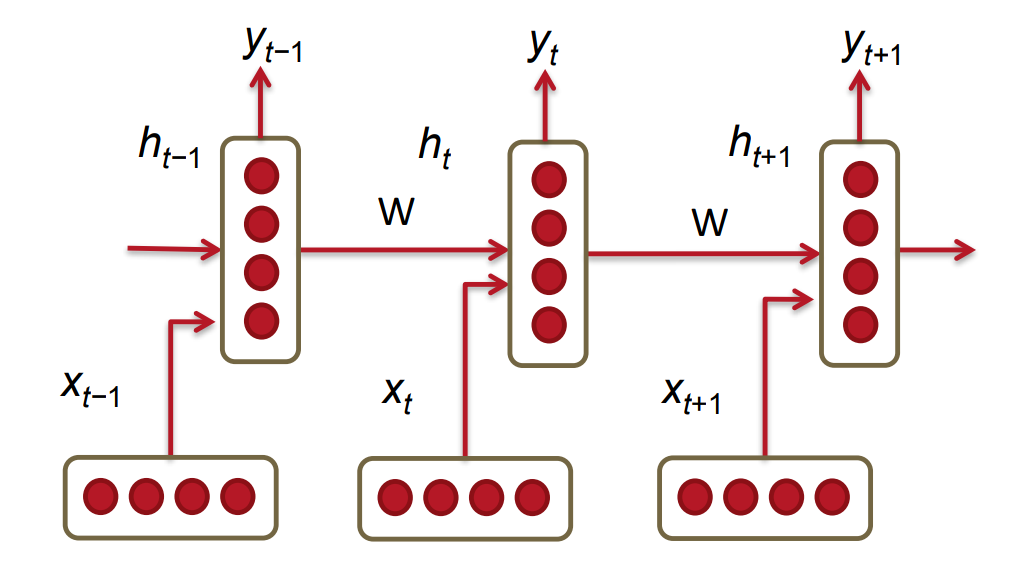
\includegraphics[scale=0.3]{rnn_arch.png}
	\caption{Arhitectura RNN \cite{cs224d_notes}}
	\label{fig:rnn_arch}
\end{figure}

Descrierea parametrilor din rețea:

\begin{itemize}
	\item $x_1, x_2, ..., x_T$ vectorii cuvintelor dintr-o secvență de lungime $T$
	\item $h_t = \sigma{(W^{(hh)} h_{t-1} + W^{(hx)} x_{[t]})}$: formula care descrie calculul vectorului de caracteristici, $h_t$, la fiecare pas $t$:
	
	\begin{itemize}
		\item $ x_t \in {\rm I\!R}^d $ vectorul cuvântului $t$
		\item $ W^{hx} \in {\rm I\!R}^{D_h \times d} $ matricea proderilor utilizată la condiționarea vectorului de intrare, $x_t$
		\item $ W^{hh} \in {\rm I\!R}^{D_h \times D_h} $ matricea proderilor utilizată la condiționarea ieșirii de la pasul anterior, $h_{t-1}$
		\item $ h_{t-1} \in  {\rm I\!R}^{D_h} $ ieșirea funcției nonlineare de la pasul anterior, $t-1$, iar $h_0 \in  {\rm I\!R}^{D_h}$ este vectorul de inițializare pentru stratul ascuns, la pasul $t=0$
		\item $ \sigma() $ funcția nonlineară  (sigmoid in acest exemplu)
	\end{itemize}

	\item $ y_t = softmax(W^{(S)} h_t) $ ieșirea care reprezintă o distribuție de probabilitate peste vocabular la fiecare pas $t$. În esență, $y_t$ este următorul cuvânt prezis, dându-se contextul de până  acum ($ h_{t-1} $) și ultimul cuvânt observat ($x_t$). Avem  $ W^{S} \in {\rm I\!R}^{|V| \times D_h} $ și $ y \in {\rm I\!R}^{|V|} $, unde $|V|$ reprezintă cardinalitatea mulțimii $V$ adică a vocabularului de cuvinte.

\end{itemize}

Funcția de cost utilizată in rețelele neuronale recurente este de obicei CE (cross entropy error).

Pentru pasul $t$:
$$
J_{(t)}(\theta) = - \sum_{j=1}^{|V|}  ytrue_{t, j} \times \log(y_{t, j})
$$

% todo sa investighez de ce nu dispare minusul, eroare in formula
Pentru toată secvența de lungime $T$ funcția de cost devine:
$$
J = - \frac{1}{T} \sum_{t=1}^{T} J_{(t)}(\theta) = - \frac{1}{T} \sum_{t=1}^{T}  \sum_{j=1}^{|V|}  ytrue_{t, j} \times \log(y_{t, j})
$$

\cite{cs224d_notes}


\subsection{Problema dispariției sau a explodării valorilor gradientului}
O RNN împarte aceeași matrice a parametrilor pentru toată secvența de intrare. Țelul unei astfel de arhitecturi este acela de a capta contextul și în cazul secvențelor de lungimi mai mari.

Considerăm ecuațiile \ref{h_t} și \ref{y_t} de mai sus la pasul $t$. Pentru a calcula eroarea unei RNN, $dE/dW$, vom însuma erorile de la fiecare pas de timp.

\begin{equation}
	\frac{\partial E}{\partial W} = \sum_{t=1}^{T} \frac{\partial E_t}{\partial W}
\end{equation}

Eroarea la fiecare pas de timp este calculată prin diferențierea ecuațiilor  \ref{h_t} și \ref{y_t}:

\begin{equation}
	\frac{\partial E_t}{\partial W} = \sum_{k=1}^{t} \frac{\partial E_t}{\partial y_t} \frac{\partial y_t}{\partial h_t} \frac{\partial h_t}{\partial h_k} \frac{\partial h_k}{\partial W}
	\label{chain_rule_E}
\end{equation}

Unde $\frac{dh_t}{dh_k}$ este derivata parțială a stării ascunse $h_t$ în raport cu toți $k$ pași de timp anteriori.

\begin{equation}
	\frac{\partial h_t}{\partial h_k} = \prod_{j=k+1}^{t} \frac{\partial h_j}{\partial h_{j-1}} = \prod_{j=k+1}^{t} W^T \times diag[f'(j_{j-1})]
	\label{chain_rule_prod}
\end{equation}

Deoarece $h \in {\rm I\!R}^{D_n}$, fiecare $\partial h_j / \partial h_{j-1}$ este matricea Jacobian pentru $h$:

\begin{equation}
	\frac{\partial h_j}{\partial h_{j-1}} = [\frac{\partial h_j}{\partial h_{j-1, 1}} ... \frac{\partial h_j}{\partial h_{j-1,  D_n}}] =\begin{bmatrix}
		\frac{\partial h_j,1}{\partial h_{j-1, 1}} & \cdots & \frac{\partial h_j,1}{\partial h_{j-1,  D_n}}	\\[0.3em]
		\vdots           & \ddots &\vdots	\\[0.3em]
		\frac{\partial h_j,D_n}{\partial h_{j-1, 1}} & \cdots & \frac{\partial h_j,D_n}{\partial h_{j-1, D_n}}
	\end{bmatrix}
	\label{jac_mat}
\end{equation}

Din \ref{chain_rule_E}, \ref{chain_rule_prod}, \ref{jac_mat} avem urmatoarea relatie:
\begin{equation}
	\frac{\partial E}{\partial W} = \sum_{t=1}^{T} \sum_{k=1}^{t} \frac{\partial E_t}{\partial y_t} \frac{\partial y_t}{\partial h_t} (\prod_{j=k+1}^{t} \frac{\partial h_j}{\partial h_{j-1}}) \frac{\partial h_k}{\partial W}
\end{equation}

Inecuația \ref{norm_ineq1} arată norma matricei Jacobian, unde $\beta_w$ și $\beta_h$ reprezintă limitele superioare ale celor doua norme ale matricelor. Norma gradientului de la fiecare pas $t$ este calculată în funcție de inecuația de mai jos.

\begin{equation}
	|| \frac{\partial h_j}{\partial h_{j-1}}|| \leq || W^T || || diag[f'(h_{j-1})]|| \leq \beta_w\beta_h
	\label{norm_ineq1}
\end{equation}

Norma L2 este folosită în aceste inecuații. Iar norma derivatei $f'(h_{j-1})$ nu poate depăși valoarea $1$, deoarece $f=sigmoid$.

\begin{equation}
	|| \frac{\partial h_j}{\partial h_k}|| = || \prod_{j=k+1}^{t} \frac{\partial h_j}{\partial h_{j-1}} || \leq (\beta_w\beta_h)^{t-k}
\end{equation}
 	
Termenul $(\beta_w\beta_h)^{t-k}$ poate foarte ușor să devină foarte mic sau foarte mare, atunci când $\beta_w\beta_h$ este mai mare ca $1$ și $t-k$ suficient de mare. Obținem valori mari pentru $t-k$ în cazul in care se dorește evaluarea funcției de criteriu pentru cuvintele (intrările) mai îndepărtate. Așadar contribuția intrărilor de la pașii inițiali se diminuează cu cât ne îndepărtăm în timp.

În timpul experimentelor s-a observat că odată ce valoare gradientului crește foarte mult, poate cauză erori de memorie (valoarea nu încape în tipul de date specificat) ceea ce rezultă în valori nedefinite (exemplu NaN (not a number)), lucru ușor detectabil la timpul rulării. Această problemă adresează explodarea valorilor gradientului(% todo de gasit o exprimare mai buna)..

Iar cea de-a doua chestiune, cea a diminuării valorii gradientului privește cazul în care valorile pentru gradient devin apropiate de zero, de multe ori acest comportament trece nedetectat, rezultând astfel o calitate mai slabă a învățării cuvintelor îndepărtate.

\subsection{Soluții pentru dispariția/explodarea gradientului}

Pentru a problema explodării gradientului, Thomas Mikolov, introduce pentru prima dată o euristică simplă - când gradientul tinde să aibă valori exagerate, ele se vor reseta la valori mici.

Referitor la problema dispariției gradientului, se folosesc de regulă două metode. Una din ele abordează modul de inițializare al parametriilor astfel că în locul unei inițializări aleatoare se folosește matricea identitate. Iar cea de-a doua tehnică propune folosirea funcției de activare ReLu (Rectified Linear Units) în detrimentul celei sigmoid. Motivul este acela că derivata funcției relu este fie 1 fie 0, iar la propagarea erorii înapoi vor fi afectați doar neuronii a căror derivată este 1.

\subsection{LSTM}



\subsection{Seq2Seq}